\section{Advanced Users: How to couple a new code}
\label{sec:newCodeCoupling}
\begin{figure}
\centering
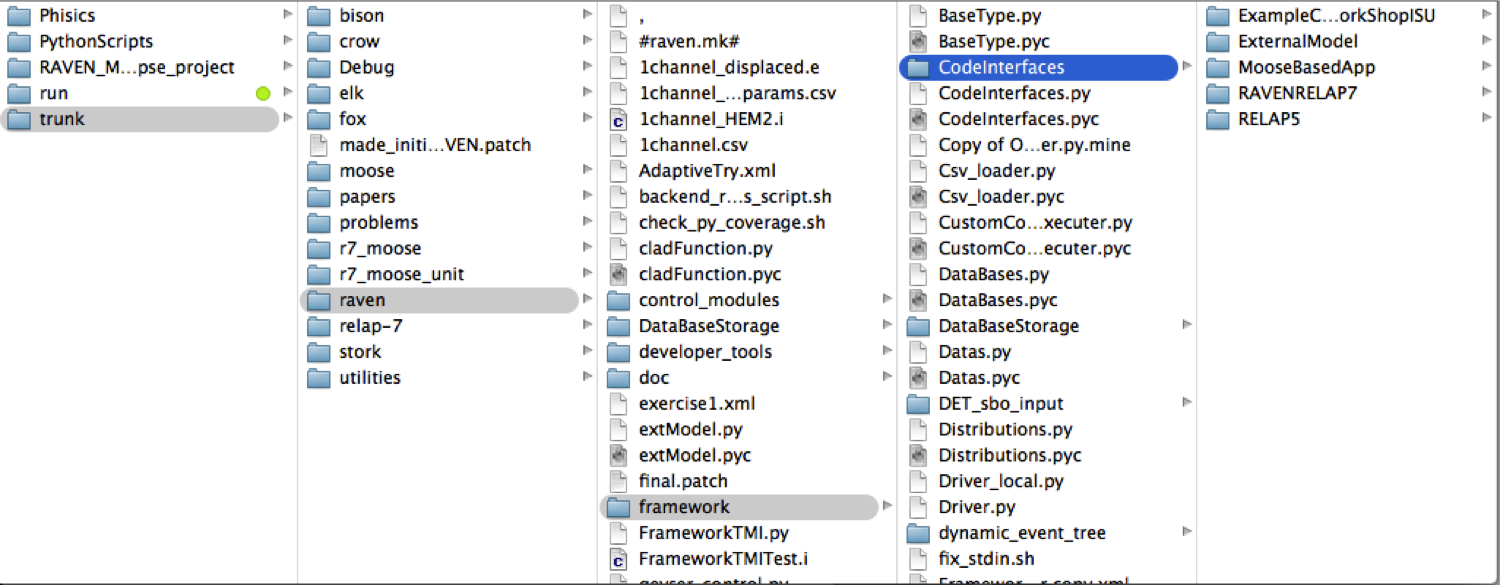
\includegraphics[width=1.0\textwidth]{pics/CodeInterfaceLocation.png}
\caption{Code Interface Location.}
\label{fig:codeinterface}
\end{figure}
The procedure of coupling a new code/application with RAVEN is a straightforward process.
For all the codes currently supported by RAVEN (e.g. RELAP-7, RELAP5-3D,
BISON, MOOSE,etc.), the coupling is performed through a Python interface that interprets the information coming from RAVEN and translates them into the
  input of the driven code.
The coupling procedure does not require modifying RAVEN itself. Instead, the developer creates a new Python interface that is going to be embedded
 in RAVEN at run-time (no need to introduce  hard-coded coupling statements).
 This interface needs to be placed in a folder (whatever name) located in (see figure~\ref{fig:codeinterface}):
\begin{lstlisting}[language=bash]
 path/to/raven/distribution/raven/framework/CodeInterfaces/
\end{lstlisting}
At the initialization stage, RAVEN imports all the Interfaces that are contained in this directory and performs some preliminary cross-checks.
\\It is important to notice that the name of class in the Interface module is the one the user needs to specify when the new interface 
needs to be used. For example, if the Interface module contains the class 	``NewCode'', the \textit{subType} in the \xmlNode{Code} block will be 	``NewCode'':
\begin{lstlisting}[language=python]
  class NewCode(CodeInterfaceBase):
    ...
\end{lstlisting}
\begin{lstlisting}[style=XML,morekeywords={name,file}] %moreemph={name,file}]
  <Models>
    ...
    <Code name='whatever' subType='NewCode'>
     ...
    </Code>
    ...
  </Models>
\end{lstlisting}
In the following sub-sections, a step-by-step procedure for coupling a code to RAVEN is outlined.
\subsection{Pre-requisites.}
\label{subsec:prerequisites}
In order to couple a newer application to the RAVEN code, some pre-requisites need to be satisfied.
%%% INPUT %%%
\newline
\\\textbf{\textit{\underline{Input}}}
\newline
\\ The first pre-requisite is the knowledge of the input
syntax of the application the developer wants to couple. Indeed, RAVEN task
 ``ends'' at the Code Interface stage. RAVEN transfers the information needed
 to perturb the input space into the Code interface and expects that the newly
 developed Interface is able to perturb the input files based on the information
 passed through.
\\This means that the developer needs to code a Python-compatible parser of
 the system code input (a module that is able to read and modify the input of
 the code that needs to be coupled).
\\ For example, let's suppose the input syntax of the code the developer needs
to couple is as follows:
\begin{lstlisting}[language=python]
  kewword1 =  aValue1
  kewword2 =  aValue2
  kewword3 =  aValue3
  kewword4 =  aValue4
\end{lstlisting}
The Python input parser would be:
\begin{lstlisting}[language=python]
class simpleInputParser():
  def __init__(self,filename):
    #
    # @ In, string, filename, input file name (with path)
    #
    self.keywordDictionary = {}
    # open the file
    fileobject = open(filename)
    # store all the lines into a list
    lines = fileobject.readlines()
    # parse the list to construct
    # self.keywordDictionary dictionary
    for line in lines:
      # split the line with respect
      # to the symbol "=" and store the
      # outcomes into the dictionary
      # listSplitted[0] is the keword
      # listSplitted[1] is the value
      listSplitted = line.split("=")
      keyword = listSplitted[0]
      value   = listSplitted[1]
      self.keywordDictionary[keyword] = value
    # close the file
    fileobject.close()

  def modifyInternalDictionary(self,inDictionary):
      #
      # @ In, dictionary {keyword:value},
      # inDictionary, dictionary containing
      # the keywords to perturb
      #

    # we just parse the dictionary and replace the
    # matching keywords
    for keyword,newvalue in inDictionary.items():
      self.keywordDictionary[keyword] = newvalue

  def writeNewInput(self,filename):
    #
    # @ In, string, filename, newer input file name (with path)
    #

    # open the file
    fileobject = open(filename)
    # write line by line
    for keyword,newvalue in self.keywordDictionary.items():
      fileobject.write(keyword + ``='' + str(newvalue) + ``\n'')
    # close the file
    fileobject.close()
\end{lstlisting}
It is important to notice that for most of the codes, a wild-card approach can be used. In case this approach fits the user's needs,
the RAVEN developer team suggests to inherit from the $GenericCode$ Interface (see section ~\ref{subsec:genericCodeInterface}).

%%% OUTPUT %%%
\textbf{\textit{\underline{Output}}}
\newline
\\RAVEN is able to handle Comma Separated Value (CSV) files (as outputs
of the system code). In order make RAVEN able to retrieve the information
 from the newly coupled code, these files need to be  either generated by the
 system code itself or the developer needs to code a Python-compatible
module to convert the whatever code output format to a CSV one.
This module can be  directly called in the new code interface (see following section).
\\ Let's suppose that the output format of the code (the same of the previous
input parser example) is as follows:
\begin{lstlisting}[language=python]
  result1 = aValue1
  result2 = aValue2
  result3 = aValue3
\end{lstlisting}
The Python output converter would be as simple as:
\begin{lstlisting}[language=python]
def convertOutputFileToCSV(outputfile):
    keywordDictionary = {}
    # open the original file
    fileobject = open(outputfile)
    outputCSVfile = open (outputfile + '.csv')
    # store all the lines into a list
    lines = fileobject.readlines()
    # parse the list to construct
    # self.keywordDictionary dictionary
    for line in lines:
      # split the line with respect
      # to the symbol "=" and store the
      # outcomes into the dictionary
      # listSplitted[0] is the keword
      # listSplitted[1] is the value
      listSplitted = line.split("=")
      keyword = listSplitted[0]
      value   = listSplitted[1]
      keywordDictionary[keyword] = value
    outputCSVfile.write(','.join(keywordDictionary.keys()))
    outputCSVfile.write(','.join(keywordDictionary.values()))
    outputCSVfile.close()
\end{lstlisting}
And the output CSV becomes:
\begin{lstlisting}[language=python]
  result1, result2, result3
  aValue1, aValue2, aValue3
\end{lstlisting}
%%%%%%%
\subsection{Code Interface Creation}
\label{subsec:codeinterfacecreation}
As already mentioned, RAVEN imports all the ``Code Interfaces'' at run-time,
without actually knowing the syntax of the driven codes. In order to make RAVEN
able to drive a newer software, the developer needs to code a Python module
that will contain few methods (with strict syntax) that are called by RAVEN during the simulation.
\\ When loading a ``Code Interface'', RAVEN expects to find, in the class representing the code,
 the following required methods:
\begin{lstlisting}[language=python]
from CodeInterfaceBaseClass import CodeInterfaceBase
class NewCode(CodeInterfaceBase):
  def generateCommand(self, inputFiles, executable, clargs=None, fargs=None)
  def createNewInput(self, currentInputFiles, oriInputFiles,
                                samplerType, **Kwargs)
\end{lstlisting}
In addition, the following optional methods can be specified:
\begin{lstlisting}[language=python]
from CodeInterfaceBaseClass import CodeInterfaceBase
class NewCode(CodeInterfaceBase):
  ...
  def finalizeCodeOutput(self, command, output, workingDir)
  def getInputExtension(self)
  def checkForOutputFailure(self, output, workingDir)
\end{lstlisting}
In the following sub-sections all the methods are fully explained, providing examples
 (referring to the simple code used as example for the previous sections)
\subsubsection{Method: \texttt{generateCommand}}
\label{subsubsec:generateCommand}
\begin{lstlisting}[language=python]
def generateCommand(self, inputFiles, executable, clargs=None, fargs=None)
\end{lstlisting}
The \textbf{generateCommand} method is used to generate the commands
(in \texttt{string} format) needed to launch the driven Code, as well as the root name of the output of the perturbed inputs (in \texttt{string} format).
The return for this command is a two-part \texttt{Python} tuple.  The first entry is a list of two-part tuples, each
which specifies whether the corresponding command
should be run exclusively in serial, or whether it can be run in parallel, as well as the command itself.
For example, for a command where
two successive commands are called, the first in serial and the second in parallel,

\begin{lstlisting}[language=python]
  def generateCommand(self,inputFiles,executable,clargs=None,fargs=None):
    . . .
    commands = [('serial',first_command), ('parallel',second_command)]
    return (commmands,outFileRoot)
\end{lstlisting}
For each command, the second entry in the tuple is a string containing the full command
that the internal JobHandler is going to use to run the Code this interface refers to.
The return data type must be a Python \texttt{tuple} with a list of tuples and a string: (\texttt{commands, outfileRoot}).
Note that in most cases, only a single command needs to be run, so only a single command tuple is necessary.
At run time, RAVEN will string together commands attached by double ampersands (\&\&), and each command
labeled as parallel-compatible will be prepended with appropriate mpi arguments.  For the example above, the
command executed will be (with \xmlNode{NumMPI} equal to 4)

\begin{lstlisting}[language=bash]
$  first_command && mpiexec -n 4 second_command
\end{lstlisting}

RAVEN is going to call the \texttt{generateCommand} function passing in the following arguments:
\begin{itemize}
  \item \textbf{\texttt{inputFiles}}, data type = list: List of input files (length of the list depends on the
           number of inputs listed in the Step which is running this code);
  \item \textbf{\texttt{executable}}, data type = string, executable name with absolute
            path \\(e.g. /home/path\_to\_executable/code.exe);
  \item  \textbf{\texttt{clargs}}, \emph{optional}, data type = dictionary, a dictionary containing the command-line flags the
               user can specify in the input (e.g. under the node $<Code><clargs type='input' arg='-i' extension='.inp'/></Code>$).
  \item  \textbf{\texttt{fargs}}, \emph{optional}, data type = dictionary, a dictionary containing the axuiliary input file variables the
               user can specify in the input (e.g. under the node $<Code><clargs type='input' arg='aux' extension='.aux'/></Code>$).
\end{itemize}
For the example referred to in the previous section, this method would be implemented as follows:
\newline
\begin{lstlisting}[language=python]
  def generateCommand(self,inputFiles,executable,clargs=None,fargs=None):
    found = False
    for index, inputFile in enumerate(inputFiles):
      if inputFile.endswith(self.getInputExtension()):
        found = True
        break
    if not found: raise IOError(
          `None of the input files has one of the following extensions: ` +
           ` `.join(self.getInputExtension()))
    outputfile = 'out~'+os.path.split(inputFiles[index])[1].split('.')[0]
    executeCommand = [('parallel',executable+ ` -i ` +os.path.split(inputFiles[index])[1])]
    return executeCommand,outputfile
\end{lstlisting}


\subsubsection{Method: \texttt{createNewInput}}
\label{subsubsec:createNewInput}
\begin{lstlisting}[language=python]
def createNewInput(self,currentInputFiles,oriInputFiles, samplerType,**Kwargs)
\end{lstlisting}
The \textbf{createNewInput} method is used to generate an input based
on the information RAVEN passes in. In this function the developer needs to
call the driven code input parser in order to modify the input file, accordingly with
respect to the variables RAVEN is providing. This method needs to return a list containing
the path and filenames of the modified input files. \nb RAVEN expects that at least one input
file of the original list gets modified.

RAVEN is going to call this function passing in the following arguments:
\begin{itemize}
  \item \textbf{\texttt{currentInputFiles}}, data type = list: List of current
              input files. This list of files is the one the code interface needs to use to print the new perturbed list of files.
              Indeed, RAVEN already changes the file location in sub-directories and the Code Interface does not need to
              change the filename or location of the files. For example, the files are going to have a absolute path as following:
              $.\textbackslash path_to_working_directory\textbackslash stepName\textbackslash anUniqueIdentifier\textbackslash filename.extension$. In case of sampling, the 
              ``\textit{anUniqueIdentifier}'' is going to be an integer (e.g. 1).
  \item \textbf{\texttt{oriInputFiles}} , data type = list, List of the original input files;
  \item  \textbf{\texttt{samplerType}} , data type = string, Sampler type (e.g. MonteCarlo,
               Adaptive, etc.). \nb None if no Sampler has been used;
  \item  \textbf{\texttt{Kwargs}} , data type = kwarded dictionary, dictionary of parameters.
               In this dictionary there is another dictionary
               called "SampledVars" where RAVEN stores the
               variables that got sampled
               (Kwargs['SampledVars'] = \{'var1':10,'var2':40\});
\end{itemize}
For the example referred in the previous section, this method would implemented as follows:
\newline
\begin{lstlisting}[language=python]
  def createNewInput(self,currentInputFiles,
        oriInputFiles,samplerType,**Kwargs):
    for index, inputFile in enumerate(oriInputFiles):
      if inputFile.endswith(self.getInputExtension()):
        break
    parser = simpleInputParser(currentInputFiles[index])
    parser.modifyInternalDictionary(**Kwargs['SampledVars'])
    parser.writeNewInput(newInputFiles[index])
    return newInputFiles
\end{lstlisting}


\subsubsection{Method: \texttt{getInputExtension}}
\label{subsubsec:getInputExtension}
\begin{lstlisting}[language=python]
def getInputExtension(self)
\end{lstlisting}
The \textbf{getInputExtension} function is an optional method. If present, it is called
by RAVEN code at run time.  This function can be considered an utility method, since its
main goal is to return a tuple of strings, where the developer can place all the input extensions
the code interface needs to support (i.e. the extensions of the input(s) the code interface
is going to ``perturb''). If this method is not implemented, the default extensions are  \textbf{(".i", ".inp", ".in"')}.
This function does not accept any input argument.
For the example referred in the previous section, this method would implemented as follows:
\newline
\begin{lstlisting}[language=python]
def getInputExtension(self):
    return (".i",".input")
\end{lstlisting}


\subsubsection{Method: \texttt{finalizeCodeOutput}}
\label{subsubsec:finializeCodeOutput}
\begin{lstlisting}[language=python]
def finalizeCodeOutput(self, command, output, workingDir)
\end{lstlisting}
The \textbf{finalizeCodeOutput} function is an optional method. If present, it is called
by RAVEN code at the end of each run. It can be used for those codes, that do not create CSV
files as output to convert the whatever output format into a CSV. RAVEN checks if a string is returned;
if so, RAVEN interprets that string as the new output file name (CSV).
\\RAVEN is going to call this function passing in the following arguments:
\begin{itemize}
  \item \textbf{\texttt{command}}, data type = string: the command used to run
                    the just ended job;
  \item \textbf{\texttt{output}}, data type = string, the Output name root;
  \item  \textbf{\texttt{workingDir}}, data type = string, current working directory.
\end{itemize}
For the example referred in the previous section, this method would implemented as follows:
\newline
\begin{lstlisting}[language=python]
def finalizeCodeOutput(self, command, output, workingDir):
    outfile = os.path.join(workingDir,output+".o")
    convertOutputFileToCSV(outfile)
 \end{lstlisting}

 \subsubsection{Method: \texttt{checkForOutputFailure}}
\label{subsubsec:checkForOutputFailure}
\begin{lstlisting}[language=python]
def checkForOutputFailure(self, output, workingDir)
\end{lstlisting}
The \textbf{checkForOutputFailure} function is an optional method. If present, it is called
by RAVEN code at the end of each run. This method needs to be implemented by the codes that, if a run fails, return a ``returncode'' = 0.
This can happen in those codes that record the failure of a run (e.g. not converged, etc.) as normal termination (returncode == 0)
This method can be used, for example, to parse the outputfile looking for a special keyword that testifies that a particular job  failed
 (e.g. in RELAP5 would be the keyword "********"). This method MUST return a boolean (True if failed, False otherwise).
\\RAVEN is going to call this function passing in the following arguments:
\begin{itemize}
  \item \textbf{\texttt{output}}, data type = string,the Output name root;
  \item  \textbf{\texttt{workingDir}}, data type = string, current working directory.
\end{itemize}
For the example referred in the previous section, this method would implemented as follows:
\newline
\begin{lstlisting}[language=python]
def checkForOutputFailure(self, command, output, workingDir):
    from  __builtin__ import any
    errorWord = "ERROR"
    return any(errorWord in x for x in
      open(os.path.join(workingDir,output+'.o'),"r").readlines())
 \end{lstlisting}

\subsection{Tools for Developing Code Interfaces}
To make generating a code interface as simple as possible, there are several tools RAVEN makes available within the Code Interface objects.

\subsubsection{File Objects}
RAVEN has created a wrapper for files within Python in order to carry along some additional information.  This allows the user to tag particular files for reference in the Code Interface, using the \xmlAttr{type} XML attribute in \xmlNode{Files} nodes.  To differentiate, RAVEN file objects will use the capital Files, whereas typical files will use the lowercase files.

When the Files are passed in to \texttt{createNewInput}, they are passed in as Files objects. To access the xmlAttr{type} of a file, use the method \texttt{getType}.  For instance, instead of looking for an extension, a Code Interface might identify an input file by looking for a particular type, as shown in the example below. \nb RAVEN does not access a File's \xmlAttr{type}; it is exclusively an optional tool for Code Interface developers.

\begin{lstlisting}[language=python,showstringspaces=false]
found = False
for inFile in inputFiles:
  if inFile.getType()=='mainInput':
    found = True
    break
if not found:
  raise IOError('Desired file with type ``mainInput'' not found!')
\end{lstlisting}
Using Files \xmlAttr{type} attributes can especially help when multiple input files have the same extension.  For example, say a Code execution command normally has the following appearance on the command line:
\begin{lstlisting}[language=bash]
/home/path/to/executable/myexec.sh -i mainInp.xml -a auxInp.xml --mesh cube.e
\end{lstlisting}
The \xmlNode{Files} block in the RAVEN XML might appear as follows:
\begin{lstlisting}[language=XML]
<Files>
  <Input name='main' type='base'>mainInp.xml</Input>
  <Input name='two'  type='aux' >auxInp.xml</Input>
  <Input name='cube' type='mesh' perturbable='False'>cube.e</Input>
</Files>
\end{lstlisting}
The search for these files in the Code Interface might then look like the example below, assuming one file per type:
\begin{lstlisting}[language=python,showstringspaces=false]
# populate a type dictionary
typesDict={}
for inFile in inputFiles:
  typesDict[inFile.getType()]=inFile
# check all the necessary files are there
if 'base' not in typesDict.keys():
  raise IOError('File type ``base'' not listed in input file!')
if 'aux' not in typesDict.keys():
  raise IOError('File type ``aux'' not listed in input file!')
if 'mesh' not in typesDict.keys():
  raise IOError('File type ``mesh'' not listed in input file!')
mainFile = typesDict['base']
# do operations on file, etc.
\end{lstlisting}

Additionally, a Code Interface developer can access the \xmlAttr{perturbable} through the \texttt{getPerturbable()} method of a Files object.  This can be useful, for example, in preventing searching binary files for variable names when creating new input. For example,
\begin{lstlisting}[language=python]
for inFile in inputFiles:
  if not inFile.getPerturbable(): continue
  # etc
\end{lstlisting}
